%===================================== CHAP 2 =================================

\chapter{Problem Description}
In Fantasy Premier League a manager attempts to maximize his total score over an entire season. For each gameweek, decisions must be made on which players to include in the squad and which players to be selected for a starting line-up. In addition, a captain- and vice-captain choice must be made. Further, one has to set a substitution priority for the players that are not selected for the starting line-up. As pointed out in Chapter \ref{introduction}, the manager is allowed to perform transfers during the season. Therefore, a manager must also decide whether to make a transfer, and which players to be transferred in and out for each gameweek.
\newpar
The FTCP consists of optimizing the decisions mentioned above for every gameweek. As new decisions are made every gameweek, the FTCP is a multi-week problem. The scope of this thesis is two-folded. Firstly, the aim is to model the FTCP. Secondly, we intend to use insights acquired from running this model with realized points in order to develop a decision support tool for human managers. 


\begin{comment}
Although the ultimate target would be to finish on top of Fantasy Premier League, winning requires a great amount of luck due to the high uncertainty in football.
The scope of this thesis is to create an optimization model that is competitive to the top rated Fantasy Premier League players. 
\end{comment}

\section{Rules of Fantasy Premier League} \label{rules of fpl}

In order to understand how the Fantasy Premier League works, it is necessary to have a review of the rules of the game. Each season consists of 380 fixtures split into a set of 38 chronological gameweeks. Each gameweek typically consists of 10 matches and features each of the English Premier League's (EPL) teams once. All the matches within a gameweek are usually played over a period of 3-4 days.

\newpar

Each player in the FPL database is assigned with a value, depending on how well the player is expected to perform. Players that are expected to score a lot of goals, create many scoring chances, or keeping a clean sheet, are often assigned with a high purchase price. Player prices change during the season dependent on the popularity of the player in the transfer market. A player's value will increase when more managers select him, and decrease when fewer managers select him. Further, a player's selling price may be less than the player's current purchase price as a sell-on fee of 50 \% (rounded down to the nearest \pounds 0.1m) will be applied on any profits made on that player. For example, if you buy a player for \pounds 9.5m and when you transfer him his price is \pounds 9.8m, his selling price will be \pounds 9.6m.

\begin{comment}
In the model there is a difference between the selected squad, the starting line-up and substitutes. The selected squad include all the players whom could be picked for the starting line-up. Further, players in the starting line-up are the ones which get credited points. Those who are not picked for the starting line-up are regarded as substitutes. Hence, the connection between these three sets is that whenever players in the starting line-up do not feature, a player from the substitutes replaces them.
\end{comment}
\newpar
Initially, one must select a team of 15 players consisting of exactly: 2 goalkeepers, 5 defenders, 5 midfielders and 3 forwards. As each EPL team has a registered squad of 25 players, the whole FPL database consists of approximately 500 players. This creates numerous ways of selecting the team. The total purchase price of the team may not exceed the initial budget limit of £100. Notice that the budget limit may vary over time, as player prices increases and decreases during the season. Further, one can not select more than three players from the same club. After the FPL manager has selected 15 players for their squad, a starting line-up consisting of 11 players has to be selected. The players in the starting line-up are the only players that get awarded points. However, if a player from the starting line-up is not playing, they will be replaced by one of the four players on the bench. You can play in any formation as long as there is 1 goalkeeper, at least 3 defenders, at least 3 midfielders and at least 1 forward. This is regarded as the team formation criteria.
\newpar
For each gameweek, the manager may use one free transfer if they want to replace one of their players with another player. It is possible to make more than one transfer for a gameweek, but each additional transfer in a gameweek will deduct 4 points from the total score. However, if the manager choose not to make any transfers for a gameweek, the free transfer is saved for the next gameweek and then it possible to make two free transfers. It is important to notice that one can not make more than two free transfers for a given gameweek. Thus, not making any transfers for two consecutive gameweeks does not give one the opportunity to make three free transfers in the upcoming gameweek. 


\begin{figure}[H]
\centering
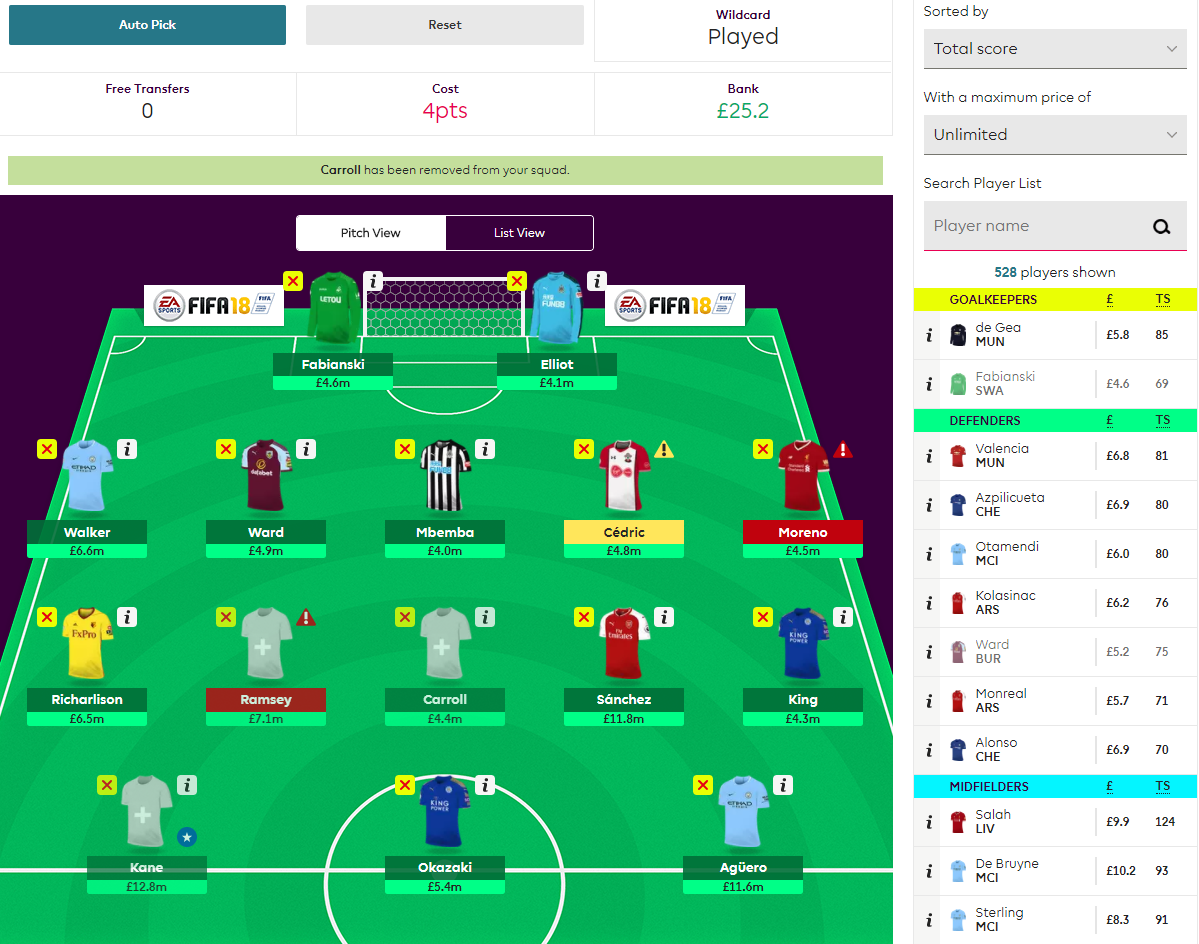
\includegraphics[scale=0.35]{fig/fantasyteam1.png}
 \captionsource{Illustration of the team selection page of Fantasy Premier League.}{https://fantasy.premierleague.com/a/squad/transfers (10.12.2017)}
\label{Figure_2.1}
\label{fig:fantasy_bilde}
\end{figure}

Figure \ref{Figure_2.1} illustrates how a squad is selected in FPL. By hitting the x-button linked to a player, one can transfer out this player. It also illustrates that the manager is considering to remove Kane, Ramsey and Carroll. As one can see, this deducts -4 points. Hence, the manager had two free transfers for this gameweek. Further, the manager has \pounds 25.2 left in the bank if these transfers are carried out. In addition, it is observed that Ramsey and Moreno have a red triangle attached to them. This implies that they are either injured or suspended for the upcoming gameweek. Notice how the squad consist of exactly 2 goalkeepers, 5 defenders, 5 midfielders and 3 forwards as stated in the game rules. 


\section{The Point System} \label{point_system}
The Premier League players are rewarded with fantasy points depending on their performance during a gameweek. The main point factors are related to goals scored, i.e. goalscorers, players with assists and players that do not concede any goals. In the following, the point system according to fantasypremierleague.com is presented. 

\begin{table}[H]
\centering
\small
\begin{tabular}{|l|l|l|l|l|}
\hline
                               & Goalkeepers & Defenders & Midfielders & Forwards \\
\hline
For playing up to 60 minutes   & 1           & 1         & 1           & 1        \\
For playing 60 minutes or more & 2           & 2         & 2           & 2        \\
For each goal scored           & 6           & 6         & 5           & 4        \\
For each assist                & 3           & 3         & 3           & 3        \\
For keeping a clean sheet      & 4           & 4         & 1           & -        \\
For every 3 saves made         & 1           & -         & -           & -        \\
For each penalty saved         & 5           & -         & -           & -        \\
For each penalty missed        & -2          & -2        & -2          & -2       \\
For every two goals conceded   & -1          & -1        & -           & -        \\
For each yellow card           & -1          & -1        & -1          & -1       \\
For each red card              & -3          & -3        & -3          & -3       \\
For each own goal              & -2          & -2        & -2          & -2      \\
\hline
\end{tabular}
\caption{Point system of FPL.}
\end{table}

\begin{itemize}
    \item In a match, the three best players are evaluated according to the FPL Bonus Points System, and are awarded a bonus of 1, 2 and 3 points. 
    \item In order for a goalkeeper or defender to receive points for a clean sheet, he has to play at least 60 minutes, excluding stoppage time. 
    \item If a goal is scored on a direct free kick or a penalty, the player that got the free kick/penalty is awarded with an assist. 
    \item For each round, you choose a captain and a vice-captain. If the captain is playing, he will be awarded with double points for the entire round. However, if the captain is not playing, your vice captain will be awarded double points. 
\end{itemize}
Notice that the point system does not consider the outcome of a match. Hence, players are not rewarded with points for playing on a team that wins or loses. 
\newpar
In addition to the regular scoring system, each manager is awarded four chips, where only one chip can be used in a gameweek: 
\begin{enumerate} [label=(\roman*)]

\item \textbf{Wildcard}. The wildcard can be used twice a season, once before New Years and once after. A wildcard allows the manager to replace his entire squad for free. As for the wildcard squad selection, the same rules applies as for the regular fantasy team composition. Hence, one can only select a maximum of three players from each team and the formation constraints must be held. When playing a wildcard, a manager's budget is set to the sell price of his original squad at that particular Gameweek. Further, when playing a wildcard, any saved transfers will be lost. One will be back to the usual 1 free transfer the following Gameweek.

\item \textbf{Bench boost}. With the bench boost you receive points for all the 15 players of your squad. The bench boost chip can only be used once. 

\item \textbf{Free hit}. The free hit chip allows the manager to replace his entire squad for one gameweek. However, for the next gameweek your original team will return.  This chip can only be used once a season. As for the wildcard chip, the same transfer- and budget rules applies for the free hit chip.

\item \textbf{Triple captain}. Triples the points of your captain for a gameweek. If the captain does not play, the triple points are awarded to the vice captain. The triple captain chip can only be used once a season. 
\end{enumerate}

